\chapter{Permutations and Combinations}
In this chapter we will study basic principles of counting, permutations and combinations. This study will enable you to further
study the branch of mathematics called combinatorics. You would have certainly encountered a combinatorical problem in your
life. It would be really surprising if you have not. Have you ever solved a Sudoku puzzle or Rubik's cube? Have you ever counted
the number of poker hands that are full houses in order to determine the odds against a full house? Have you ever attempted to
trace through a network without removing your pencil from paper and without tracing any part of network more than once? These are
all combinatorical problems. As you can see that combinatorics has evolved from mathematical games.

With the invention of modern computers, we are enabled to solve more and more problems of combinatorics which were earlier not
feasible due to calculations involved. The computer programs are often based on combinatorical algorithms which determine the speed
and efficiency of the solution. Analysis of these programs and algorithms require sound knowledge of combinatorical mathematics and
thinking. In computer science we write test cases for our programs, and those test cases can be enumerated by applying permutations
and combinations on input data and states produced in the program. Combinatorics is a powerful tool for making sure that the tester
does not miss any test case, which in mission-critical programs is of paramount importance.

The best way to learn combinatorics is to solve a lot of problems. This is in general true for all branches of mathematics but even
more so for combinatorics because a problem which appears simple may be quite difficult to solve or require critical thinking. By
solving problems of different kinds, and by repeating them the concepts will be enforced and discipline will develop.

We start with four basic counting principles and then we will progress into permutations and combinatins. To study the topic of
permutations and combinations it is required to have basic knowledge in set theory which the reader is expected to know.

\section{Four Basic Counting Principles}
Let $S$ be a set. A \textit{partition} of $S$ is a collection of $S_1, S_2, \ldots, S_m$ of subsets of $S$ such that each element
in $S$ is in exactly one of these subsets:
$$S = S_1\cup S_2\cup\ldots\cup S_m$$
$$S_i\cap S_j = \phi(i\neq j)$$
Thus, the sets $S_1, S_2, \ldots, S_m$ are pairwise disjoint sets, and their union is $S$. The subsets $S_1, S_2, \ldots, S_m$ are
called the \textit{parts} of the partition. Note that by this definition a part of the partition may be empty, but usually there is
no advantage in considering partitions with one or more empty sets. The number of objects of a set $S$ is denoted by $|S|$, and is
called the \textit{size} of $S$.

\subsection{Addition Principle}
Suppose that a $S$ is partitioned into pairwise disjoint partys $S_1, S_2, \ldots, S_m$. The number of objects in $S$ can be
determined by finding the number of objects in each of the parts, and adding the numbers so obtained:
$$|S| = |S_1| + |S_2| + \ldots |S_m|$$.
If the sets $S_1, S_2, \ldots, S_m$ are allowed to overlap, then a more profound principle, the inclusion-exclusion principle can
be used to count the number of objects in $S$.

We need to be careful when partitioning $S$ into too many parts. For example, if we partition $S$ into parts in such a way that
each part contains only one element then addition princinple is becomes counting the number of parts, which is basically same as
listing all objects of $S$. Thus the art of applying addition princinple is to partition the set $S$ into not too many parts.

\noindent\textbf{Example:} In a university there are four mathematics courses, two economics courses, and three lietrature
courses. A student is allowed to enroll into one course at most. Thus, we see that a student can take a course in $4 + 2 + 3 = 9$
ways.

Next principle is multiplication principle which will be stated for two sets, but it can be generalized to any finite number of
sets.

\subsection{Multiplication Principle}
Let $S$ be a set of ordered pairs $(a, b)$, where the first object comes from a set of size $p$, and for each choice of object $a$
there are $q$ choices for object $b$. Then the size of $S$ is $p\times q$:
$$|S| = p\times q$$
As in basic arithmetic multiplication is repeated addition, similarly multiplication principle is actuallly a consequence of the
addition principle i.e. repeated addition. Let $a_1, a_2, \ldots, a_p$ be $p$ different choices for the object $a$. We partition
$S$ into parts $S_1, S_2, \ldots, S_p$ where $S_i$ is the set of ordered pairs in $S$ with first object $a_i(i = 1, 2, \ldots,
p)$. The size of each $S_i$ is $q$; hence, by the addition principle,
$$|S| = |S_1| + |S_2| + \ldots + |S_p|$$
$$= q + q + \ldots + q(p q'\text{s})$$
$$= p\times q$$
The multiplication principle can be stated in another way as: If a first task has $p$ outcomes, and no matter what the outcome of of
the first task, a second task has $q$ outcomes i.e. outcomes for two tasks are mutually exclusive, then the two tasks can be
performed in $p\times q$ outcomes.

\noindent\textbf{Example:} Pencil comes in two different lengths, four different hardness, and three different thickness. How many
different types of pencils are there?

The pencil has three different properties, which are exclusive of each other, and thus, we can apply multiplication
principle. Hence, number of different types of pencils is $2\times4\times3 = 24$.

\noindent\textbf{Example:} The number of ways a man, woman, boy, and girl can be selected from three men, three women, five boys and
four girls is $3\times3\times5\times4 = 180$.

\noindent\textbf{Example:} Determine the number of positive integers that are factors of the number
$$2^3\times3^4\times5^5\times7^7$$
The numbers $2, 3, 5,$ and $7$ are prime numbers. By the fundamental theorem of arithmetic, each factor is of the form
$$2^i\times3^j\times5^k\times7^l$$
where $0\leq i\leq2, 0\leq j\leq3, 0\leq k\leq5,$ and $0\leq l\leq7$. There are three choices for $i$, four for $j$, six for $k$, and
eight for $l$. By multiplication principle, the number of factors is $3\times4\times6\times8 = 576$.

In the multiplication principle the $q$ choices for object $b$ may vary with the choices of $a$. The only requirement is that there
be the same number $q$ of choices, not necessarily the same choices.

\noindent\textbf{Example:} How many two-digit numbers have distinct, and nonzero digits?

A two-digit number $ab$ can be regarded as an ordered pair $(a, b)$, where $a$ is the tens digit, and $b$ is the units digit. Both
are not allowed to be $0$, and they must be different. Thus, we see that there are $9$ ways to choose $a$, which are $1, 2, \ldots,
9$. Once $a$ is chosen we cannot use the same digit for $b$, which means we are left with $8$ choices for $b$. Here we see that
choice of $a$ makes a difference on what choices $b$ has. However, for multiplication principle to be applicable what matters is
that the number of choices remain constant which is $8$ in this case. Applying multiplication principle, we arrive at the answer of
the question as $9\times8 = 72$.

There is another way to arrive at the same result. Total number of two-digit number is $90, 10,11, 12, \ldots, 99$. Of these $90$
numbers $9$ have a zero in them$(10, 20, 30, \ldots, 90)$, and $9$ have repeated digits$(11, 22, \ldots, 99)$. Thus, total number of
required numbers equals $90 - 9 - 9 = 72$.

We can derive two important ideas from the previous example. First is that it is possible to solve a counting problem in many
ways. The second idea is that to find the number of objects in a set $A$ (in this csae the set of two-digit numbers with nonzero,
and distinct digits) it may be easier to find the number of objects in a larger set $U$ containing $S$ (the set of all
two-digit numbers), and then subtract the number of objects of $U$ that do not belong to $A$ (the two-digit numbers containing $0$
or repeated digit). This leads us to subtraction principle.

\subsection{Subtraction Principle:}
Let $A$ be a set, and let $U$ be a larger set containing $A$. Let
$$\overline{A} = U\textbackslash A = \{x\in U: x\notin A\}$$
be the complement of $A$ in $U$. Then the numebr $|A|$ of object in $A$ is given by the rule
$$|A| = |U| - |\overline{A}|$$

The set $U$ is usually some natural set containing all the objects under discussion (it is called \textit{universal set}). Using
the subtraction principle should be used only if it is easier to count the number of object in $U$ nd $\overline{A}$ tha to count the
number of objects in $A$.

\noindent\textbf{Example:} Most websites on internet have a lower limit of $8$ characters as password length. Suppose if these
passwordss are to made up of the digits $0, 1, 2, \ldots, 9$, and the lowercase letters $a, b, c, \ldots, z$ then how many passwords
will have a repeated symbol?

There are a total of $10$ digits, and $26$ letters i.e. 36 symbols. So by two applications of multiplication principle, we get
$$|U| = 36^8 = 2,821,109,907,456$$
and
$$|\overline{A}| = 36.35.34.33.32.31.30.29 = 1,220,096,908,800$$
Therefore,
$$|A| = |U| - |\overline{A}| = 1,601,012,998,656$$.

Now we will formulate the last principle of counting principles.

\subsection{Division Principle}
Let $S$ be a finite set that is partitioned into $k$ parts in such a way that each part contains the same number of objects. Then
the number of parts in the partition is given by the rule
$$k = \frac{|S|}{\text{number of objects in a part}}$$

\noindent\textbf{Example;} There are $240$ rats in a collection of cages. If each cage contains $2$ rats, the number of cages
equals $$\frac{240}{2} = 120$$.

Interesting problems of division principle will be found in the problems section.

Most counting problems can be classified as one of the following types:

\begin{enumerate}
\item Count the number of ordered arrangements or ordered selection of objects
  \begin{enumerate}
  \item without repeating any object,
  \item with repetion(perhaps limited) of objects permitted.
  \end{enumerate}
\item Count the number of unordered arrangements or unordered selection of objects
  \begin{enumerate}
    \item without repeating any object,
  \item with repetion(perhaps limited) of objects permitted.
  \end{enumerate}
\end{enumerate}

We can represent repetition, and nonrepetition of objects as selection from a set, and a multiset. The latter might prove to be more
useful in some cases. A \textit{multiset} is like a set except that its members need not be distinct.\footnote{Thus, a cardinal
rule of sets is broken by multisets because a set is not supposed to have duplicates or repeated elements. The set $\{a, a, b\}$ is
same as the set $\{a, b\}$ but not so for multisets} For example, a multiset $M$ with three $a$'s, two $b$'s i.e. $5$ elements of
$2$ different types. We usually indicate a multiset by specifying the number of times different types of elements occur in
it. Thus, $M$ is denoted by $\{3.a,2.b\}$.\footnote{In standard set-theory's notation, we could denote the multiset $M$ using
ordered pairs as $\{(a, 3), (b, 2)\}$}. The numbers $3$, and $2$ are the \textit{repetition members} of the multiset $M$. Thus we
can extrapolate that a set is a multiset with all repetition numbers equal to $1$. Often there is no limit on number of repetitions
i.e. infinite repetitions are allowed.\footnote{In no circumstance, we need to consider different sizes of $\infty$.}

\section{Factorial of $n$}
Factorial of $n$ is denoted by $n!$. In the old style it is written as $\oldfact{n}$. $n!$ is given by the first $n$ natural
numbers, i.e. $$n! = 1.2.3.4\ldots(n - 1).n$$ Also, $0! = 1$, which we will prove later.

Permutation means arrangement of objects along with selection. In the permutation of object order matter. If order of object
changes then their permutation also changes. Combination of objects means selection of objects in such a way that order does not
matter.

\section{Permutation of Sets}
Let $r\in \mathbb{P}$. By an $r$-\textit{permutation} of a set $S$ of $n$ elements has a meaning of an ordered(by definition of
permutation) arrangement of $r$ of the $n$ elements$(r\leq n)$. If $S = \{a, b, c\},$ then the three $1$-permutations of $S$ are
$$a~~~b~~~c,$$
the six $2$-permutations of $S$ are
$$ab~~~ac~~~ba~~~bc~~~ca~~~cb,$$
and the six $3$-permutations of $S$ are
$$abc~~~acb~~~bac~~~bca~~~cab~~~cba.$$

There are no $4$-permutations of $S$ because that will violate the assumption that $r\leq n$.

The $r$-permutations of an $n$-element set is denoted by $P(n, r)$ or ${}_nP_r$ or ${}^nP_r$. If $r > n$ then ${}^nP_r =
0$. Clearly, ${}^nP_1 = n$ for each $n\in \mathbb{P}$.

For $n$ and $r$ positive integers with $r\leq n,$ $${}^nP_r = n\times(n - 1)\times\ldots\times(n - r + 1).$$

Permutation of $n$ objects taken $r$ at a time is equivalent ot filling $r$ different vacant spots from $n$ different objects. We
can fill first spot by $n$ ways, second spot can be filled by remaining objects i.e. $n - 1$ ways, and proceeding this way we find
that $r$th spot can be filled in $n - r + 1$ ways. Thus total number of ways is $$n\times(n - 1)\times\ldots(n - r + 1)$$.

We can rewrite the above as $$\frac{n\times(n - 1)\ldots(n - r + 1)\times(n - r)\times\ldots2\times 1}{(n - r)\times(n - r -
  1)\times\ldots2\times1}$$
$${}^nP_r = \frac{n!}{(n - r)!}$$

Alternatively, first place can be filled in $n$ ways. Rest of $r - 1$ spots from $n - 1$ objects can be filled in ${}^{n - 1}P_{r -
1}$ ways. Thus, ${}^nP_r = n.{}^{n - 1}P_{r - 1}$. Similarly, ${}^{n - 1}P_{r - 1} = (n - 1).{}^{n - 2}P_{r - 2}$. Proceeding this
way we find that ${}^{n - r + 1}P_1 = n - r + 1$. Multiplying and cancelling common factors, we get ${}^nP_r = n\times(n -
1)\times\ldots\times(n - r + 1).$

The number of permutations of $n$ elements is ${}^nP_n = \frac{n!}{0!} = n!$. If we follow first result then it is evident that $0!
= 1.$

\subsection{Meaning of $\frac{1}{(-k)!}, k\in\mathbb{P}$}
We have ${}^nP_r = \frac{n!}{(n - r)!}$. Putting $r = n + k$, we have ${}^nP_{n + k} = \frac{n!}{(-k)!}$. But the number of ways of
arranging $n + 1$ objects out of $n$ different objects $= 0 \Rightarrow \frac{1}{(-k)!} = 0.$

\noindent\textbf{Note:} Although $(-k)!$ has no meaning by the definition of factorial but if we consider the above result then the
formula for permutation becomes valid even for $r > n.$

\subsection{Circular Permutation}
Let us consider arranging objects along a circle. Let us consider that four persons $A, B, C,$ and $D$ are sitting around a table. We
can have following arrangements:

\begin{center}
  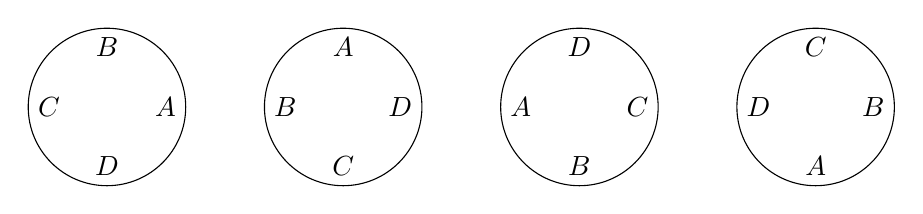
\begin{tikzpicture}
    \draw (0,0) circle (1cm);
    \draw (3cm,0) circle (1cm);
    \draw (6cm,0) circle (1cm);
    \draw (9,0) circle (1cm);
    \draw (1cm, 0) node[anchor=east] {$A$};
    \draw (0, 1cm) node[anchor=north] {$B$};
    \draw (-1cm, 0) node[anchor=west] {$C$};
    \draw (0, -1cm) node[anchor=south] {$D$};
    \draw (4cm, 0) node[anchor=east] {$D$};
    \draw (3cm, 1cm) node[anchor=north] {$A$};
    \draw (2cm, 0) node[anchor=west] {$B$};
    \draw (3cm, -1cm) node[anchor=south] {$C$};
    \draw (7cm, 0) node[anchor=east] {$C$};
    \draw (6cm, 1cm) node[anchor=north] {$D$};
    \draw (5cm, 0) node[anchor=west] {$A$};
    \draw (6cm, -1cm) node[anchor=south] {$B$};
    \draw (10cm, 0) node[anchor=east] {$B$};
    \draw (9cm, 1cm) node[anchor=north] {$C$};
    \draw (8cm, 0) node[anchor=west] {$D$};
    \draw (9cm, -1cm) node[anchor=south] {$A$};
  \end{tikzpicture}
\end{center}

As shown four persons are sitting around a round table, and four anticlockwise rotations have lead to four arrangements. But if
$A,B,C,D$ are sitting in a row, and then are shiftedd such that last occupies the place of first, then the four arrangements will be
different. Thus, if there are $n$ objects then for each circular arrangement there are nn linear arrangements. But for $n$ different
objects total number of linear arrengements are $n!$ so the total number of circular arrangements are $$\frac{n!}{n} = (n - 1)!$$.

Thus, we can say that number of circular $r$-permutations of a set of $n$ elements is given by $$\frac{{}^nP_r}{r} = \frac{n!}{r.(n
  - r)!}$$

\subsection{Clockwise and Anti-Clockwise Arrangements}
When clockwise and anticlockwise arranegemnts are same then total number of permutations will become half of what we computed in
previous case i.e. $$\frac{{}^nP_r}{2r} = \frac{n!}{2r.(n - r)!}$$

\section{Combination of Sets}
Consider a set $S$ having $n$ elements. A \textit{combination} of a set $S$ has a meaning of an unordered selection of the elements
of $S$. The result of each selection is a \textit{subset} $A$ of the elements of $S: A\subset S$. Thus, the terms
\textit{combination} and \textit{subset} are interchangeable.

Now let $r$ be a nonnegative integer. By an $r$-\textit{combination} of a set $S$ of $n$ elements, we understand an unordered
selection of $r$ of the $n$ objects of $S$. The result will be an $r$-subset of $S$.

If $S = \{a, b, c, d\},$ then $$\{a, b, c\}, \{a, b, c\}, \{a, c, d\}, \{b, c, d\}$$ are the four $3$-subsets of $S$. We denote
the number of $r$-subsets or $r$-combinations of an $n$-element set by ${n\choose r}$ or ${}_nC_r$ or ${}^nC_r$. Obviously,
$${n\choose r} = 0~~~~~~\text{if~}r > n.$$
Also,
$${0\choose r} = 0~~~~~~\text{if~}r > 0.$$

The following facts are easy to figure out for each nonnegative integer $n$ $${0\choose 0} = {n\choose 0} = {n\choose n} = 1, {n\choose 1} = n,$$

For $0\leq r\leq n,$ $${}^nP_r = r!{}^nC_r.$$
Hence,
$${}^nC_r = \frac{n!}{r!(n - r)!}$$

Let $S$ be an $n$-element set. Each $r$-permutation of $S$ arises from following tasks
\begin{enumerate}
\item Choose $r$ elements from $S$.
\item Arrange the chose $r$ elements in some order.
\end{enumerate}

The number of ways to carry out first task, by definition, is ${}^nC_r$. The number of ways to carry out second task is ${}^nP_r =
r!$. By the multiplication principle, we have ${}^nP_r = r!{}^nC_r$. Now applying the formula for permutations, we have
$${}^nC_r = \frac{n!}{r!(n - r)!}.$$

\section{Permutation of Multisets}
Let $S$ be a multiset with objects of $k$ different types, where each object can be repeated infinitely. Then the number of
$r$-permutations of $S$ is $k^r$.

To prove this, we can choose the first item to be an object of any one of the $k$ types. Since the number of repetitions are
infinite the second item can be also chose in $k$ ways. In fact, any item can be chosen in $k$ ways due to infinite
repetition. Following, multiplication principle, total number of such permutations is $k^r$.

Let $S$ be a multiset with objects of $k$ different types with finite repetition numbers $n_1, n_2, \ldots, n_k$ respectively. Let
the size of $S$ be $n = n_1 + n_2 + \ldots + n_k.$ Then the number of permutations of $S$ equals $$\frac{n!}{n_!!n_2!\ldots
  n_k!}.$$

We can calculate this by thinking in terms of $n$ places, and we want to put exactly one of the objects of $S$ in each of the
places. We have $n_1$ objects of one type in $S$, so we must choose a subset of $n_1$ places from the set of $n$ places. We can do
this in ${}^nC_{n_1}$ ways. After this we have $n - n_1$ places left, and we have $n_2$ objects of second type. So following
similarly we can do this in ${}^{n - n_1}C_{n_2}$ ways. Following this way invoking multiplication principle, the number of
permutations of $S$ equals
$${}^nC_{n_1}.{}^{n - n_1}C_{n_2}.{}^{n - n_1 - n_2}C_{n_3}\ldots{}^{n - n_1 - n_2 - \ldots - n_{k - 1}}C_{n_k}$$
which gives
$$\frac{n!}{n_1!(n - n_1)!}.\frac{(n - n_1)!}{n_2!(n - n_1 - n_2)!}.\frac{(n - n_1 - n_2)!}{n_3!(n - n_1 - n_2 -n_3)!}\ldots
\frac{(n - n_1 - n_2 - \ldots - n_{k - 1})!}{n_k!(n - n_1 - n_2 - \ldots - n_k)!}$$
which after cancellation, reduces to
$$\frac{n!}{n_1!n_2!\ldots n_k!}$$

Let $n$ be a positive integer, and let $n_1, n_2, \ldots, n_k$ be positive integers with $n = n_1 + n_2 + \ldots + n_k$. The number
of ways to partition a set of $n$ objects into $k$ labeled boxes in which Box 1 contains $n_1$ objects, Box 2 contains $n_2$
objects, $\ldots$, Box $k$ contains $n_k$ objects equals
$$\frac{n!}{n_1!n_2!\ldots n_k!}.$$

If the boxes are not labeled, and $n_1 = n_2 = \ldots = n_k$, then the number of partitions equals $$\frac{n!}{k!n_1!n_2!\ldots
  n_k!}.$$

We can calculate this by direct application of the multiplication principle. So we first choose $n_1$ objects for the first box,
then $n_2$ of the remaining $n - n_1$ objects for the second box and so on. By the multiplication principle, the number of ways is
$${}^nC_{n_1}.{}^{n - n_1}C_{n_2}.{}^{n - n_1 - n_2}C_{n_3}\ldots{}^{n - n_1 - n_2 - \ldots - n_{k - 1}}C_{n_k}$$
which is same as the last result, i.e.
$$\frac{n!}{n_1!n_2!\ldots n_k!}$$

If boxes are not labeled and $n_1 = n_2 = \ldots = n_k,$ then the result has to be divided by $k!$ because for each way of
distributing the objects into the $k$ unalbeled boxes there are $k!$ ways in which we can attach the labels to the boxes. Thus,
using the division principle, we arrive at the result as
$$\frac{n!}{n_1!n_2!\ldots n_k!}.$$

\section{Combination of Multisets}
If $S$ is a multiset, then an $r$-combination of $S$ is an unorndered selection of $r$ of the objects of $S$. Thus, an
$r$-combination of $S$ is itslef a multiset, a \textit{submultiset} of $S$ of size $r$, or, for short, an $r$-submultiset. If $S$
has $n$ objects, then there is only one $n$-combination of $S$, namely, $S$ itself. If $S$ contains objects of $k$ different types,
then there are $k 1$-combinations of $S$.

Let $S$ be a multiset with objects of $k$ types, each with an infinite repetitions, then the number of $r$-combinations of $S$
equals
$${}^{r + k - 1}C_r = {}^{r + k - 1}C_{k - 1}.$$

Let $k$ types of objects of $S$ be $a_1, a_2, \ldots, a_k$ so that
$$S = \{\infty.a_1, \infty.a_2, \ldots, \infty.a_k\}$$

Any $r$-combination of $S$ is of the form $\{x_1.a_1, x_2.a_2, \ldots, x_k.a_k\}$, where $x_1, x_2, \ldots, x_k$ are nonnegative
integers with $x_1 + x_2 + \ldots + x_k = r$. The converse is also true. Thus, the number of $r$-combinations of $S$ equals the
number of solutions of the equation $$x_1 + x_2 + \ldots + x_k = r.$$

We will show that the number of solutions of this equation is given by number of permuations of the multiset
$$T = \{r.1, (k - 1).*\}$$
of $r + k - 1$ objects of two different types. Given a permuation of $T,$ the $k - 1 *$'s divide the $r 1$s into $k$ groups. Let
there be $x_1 1$s to the left of the first $*, x_2 1$s between the first and second $*,\ldots,$ and $x_k 1$s to the right of last
$*$. Clearly, $x_1 + x_2 + \ldots + x_k = r$. The converse of this is also true. Thus, required combination is given by the
formula $${}^{r + k - 1}C_r = {}^{r + k - 1}C_{k - 1}.$$

\section{Some Important Indentities}
\begin{enumerate}
\item ${}^nP_r = r.{}^{n - 1}P_{r - 1} + {}^{n - 1}P_r$.
\item ${}^nC_r = {}^nC_{n - r}$.
\item ${}^nC_{r - 1} + {}^nC_r = {}^{n + 1}C_r$.
\item ${}^nC_r = {}^nC_s \Rightarrow r = s$ or $r + s = n$.
\item ${}^nC_r = \frac{n - r + 1}{r}.{}^nC_{r - 1}~(1\leq r\leq n)$.
\item If $n$ is even, then the greatest value of ${}^nC_r$ is ${}^nC_m$, where $m = n/2$. If $n$ is odd, then the greatet value is
  ${}^nC_m$, where $m = (n - 1)/2$ or $m = (n + 1)/2$.
\item If $n = 2m + 1$, then ${}^nC_0 < {}^nC_1 < {}^nC_2 < \ldots < {}^nC_m = {}^nC_{m + 1}$. ${}^nC_{m + 1} > {}^nC_{m + 2} >
  \ldots > {}^nC_n$.
\item If $n = 2m + 1$, then ${}^nC_0 < {}^nC_1 < {}^nC_2 < \ldots <{}^nC_m > {}^nC_{m + 1} > {}^nC_{m + 1} > \ldots > {}^nC_n$.
\item ${}^nC_0 + {}^nC_1 + {}^nC_2 + \ldots + {}^nC_n = 2^n$.
\item ${}^nC_0 + {}^nC_1 + {}^nC_2 + \ldots = {}^nC_1 + {}^nC_3 + \ldots = 2^{n -1}$.
\item ${}^{2n + 1}C_0 + {}^{2n + 1}C_1 + \ldots + {}^{2n + 1}C_n = {}^{2n + 1}C_{n + 1} = {}^{2n + 1}C_{n + 1} + {}^{2n + 1}C_{n +
  2} + \ldots + {}^{2n + 1}C_{2n + 1} = 2^{2n}$.
\item $r.{}^nC_r = n.{}^{n - 1}C_{r - 1}$.
\end{enumerate}

\section{Some Useful Results}
Number of selections of $r$ objects out of $n$ different objects:

\begin{enumerate}
\item When $p$ paticular objects are always included $= {}^pC_p.{}^{n - p}C_{r - p} = {}^{n - p}C_{r - p}$.
\item When $p$ paticular objects are excluded $= {}^{n - p}C_r$.
\item Number of selections of $r$ objects out of $n$ different objects such that $p$ particular objects are not together in any
  selection $= {}^nC_r = {}^{n - p}C_{r - p}$.
\item Number of selection of $r$ consecutive objects out of $n$ objects in a row $= n - r + 1$.
\item Number of selection of $r$ consecutive objects out of $n$ objects along a circle $= n$ when $r < n, 1$ when $r = n$.
\item Number of selections of zero or more objects out of $n$ different objects $= {}^nC_0 + {}^nC_1 + {}^nC_2 + \ldots + {}^nC_n =
  2^n$.
\item Number of selections of one or more objects out of $n$ different objects $= {}^nC_1 + {}^nC_2 + \ldots + {}^nC_n = 2^n - 1$.
\item Number of selections of zero or more objects out of $n$ identical objects $= n + 1$.
\item Number of selections of one or more objects out of $n$ identical objects $= n$.
\item Number of selection of one or more objects from $(p + q + r)$ objects, out of which $r$ objects are identical and of one
  type, $q$ objects are identical and of second type, $r$ objects are identical and of third type $= (p + 1)(q + 1)(r + 1) - 1$.
\item Number of selection of one or more objects from $(p + q + r + n)$ objects, out of which $r$ objects are identical and of one
  type, $q$ objects are identical and of second type, $r$ objects are identical and of third type and rest $n$ are different $= (p
  + 1)(q + 1)(r + 1)({}^nC_0 + {}^nC_1 + {}^nC_2 + \ldots + {}^nC_n) - 1 = (p + 1)(q + 1)(r + 1)2^n - 1$
\item Number of ways of distributing $n$ different objects among $3$ persons such that they gey $x, y, z$ objects $= {}^nC_x.{}^{n
  - x}C_y.{}^{n - x - y}C_z.3! = \frac{n!}{x!y!z!}.3!$.
\item Number of ways of distributing $n$ different objects in $5$ sets having $a, b, c, d, e$ objects$(a + b + c + d + d = n)$:
  \begin{enumerate}
  \item When two sets have equal number of objects and three sets have equal number of objects $= \frac{n!}{a!b!c!d!e!2!3!}$
  \item When all sets have equal number of objects $= \frac{n!}{a!b!c!d!e!5!}$
  \end{enumerate}
\item Number of ways of distributing $n$ different objects among $5$ persons
  \begin{enumerate}
  \item When all person get different number of objects $= \frac{n!}{a!b!c!d!e!}.5!$.
  \item When two persons get equal number of objects and three get equal number of objects $= \frac{n!}{a!b!c!d!e!2!3!}.5!$.
  \item When all get equal number of objects $= \frac{n!}{a!b!c!d!e!5!}.5! = \frac{n!}{a!b!c!d!e!}$.
  \end{enumerate}
\end{enumerate}

\section{Permutations with Repetitions}
The objective is to find permutation of $r$ objects out of $n$ objects of which $p$ are of one type, $q$ of second type and so on.

Let the different objects be denoted by $a, b, c, \ldots$

Consider the product $$\left(1 + \frac{ax}{1!} + \frac{a^2x^2}{2!} + \ldots + \frac{a^px^p}{p!}\right)\left(1 + \frac{bx}{1!} +
\frac{b^2x^2}{2!} + \ldots + \frac{b^qx^q}{q!}\right)\ldots$$

Required number of permutations $=$ sum of all possible terms of the form $= \frac{r!}{p!q!\ldots}a^pb^q\ldots$ where $p + q + \ldots
= r$

$= r!$. coeff. of $x^r$ in $\left[\left(1 + \frac{x}{1!} + \frac{x^2}{2!} + \ldots + \frac{x^p}{p!}\right)\left(1 + \frac{x}{1!} +
\frac{x^2}{2!} + \ldots + \frac{x^q}{q!}\right)\ldots\right]$

\section{Combinations with Repetitions}
The objective is to find combinations of $r$ objects out of $n$ objects under different cases of repetitions. To begin with we
consider combinations of $r$ objects taken out of $n$ objects of which $p$ are of one type, $q$ of the second type and so on.

Let the different things be denoted by the letters $a, b, \ldots$

Consider the product $(1 + ax + a^2x^2 + \ldots + a^px^2)(1 + bx + b^2x^2 + \ldots + b^qx^2)\ldots$ All the terms in the product
is of the same degree in the letters $a, b, \ldots$ as in $x$. The coefficient of $x^r$ in the product is the number of ways of
taking $r$ of the letters $a, b, \ldots$ with the restriction that maximum number of $a$'s is $p$, maximum number of $b$'s is $q$ and so
on. Coeff. of $x^r$ will not change if $a = b = \ldots = 1$. Thus required number of combinaitons = Coeff. of $x^r$ in $(1 + x + x^2 +
\ldots + x^2)(1 + x + x^2 + \ldots + x^2)\ldots$

Similarly, number of combinaitons of $r$ objects out of $n$ objects of which $p$ are of one type, $q$ are of second type and $(n -
p - q)$ things are all different $=$ Coeff. of $x^r$ in $[(1 + x + x^2 + \ldots + x^p)(1 + x + x^2 + \ldots + x^q)(1 + x)(1 +
  x)\ldots \text{~to~} (n - p - q)\text{factors~}]$

$=$ Coeff. of $x^r$ in $[(1 + x + x^2 + \ldots + x^p)(1 + x + x^2 + \ldots + x^q)(1 + x)(1 + x)^{n - p - q}]$

Similarly, number of combinations of $r$ objects out of $n$ objects of which $p$ are of one type, $q$ are of second type and so on,
when each thing is taken at least once $=$ Coeff. of $x^r$ in $[(x + x^2 + \ldots + x^p)(x + x^2 + \ldots + x^q)\ldots]$

$=$ Coeff. of $x^{r - 3}$ in $[(1 + x + x^2 + \ldots + x^p)(1 + x + x^2 + \ldots + x^q)$

If $n$ is a negative integer, then $(1 + x)^n = 1 + \frac{n}{1!}x + \frac{n(n - 1)}{2!}x^2 + \ldots\text{~to~}\infty$ [this comes
  from binomial theorem]

So if $n$ is a positive inetger then $(1 + x)^{-n} = 1 + \frac{n}{1!}x + \frac{n(n + 1)}{2!}x^2 + \ldots\text{~to~}\infty$

Coeff. of $x^r$ in $(1 - x)^{-n} = {}^{n + r - 1}C_r$ which is number of ways in which $r$ identical objects can be distributed
among $n$ persons can get zero of more objects $=$ Coeff. of $x^r$ in $(1 + x + \ldots + x^r)^n = \left(\frac{1 - x^{r + 1}}{1 -
    x}\right)^n = [(1 - x^{r + 1})(1 - x)^{-n}]$.

$=$ Coeff. of $x^r$ in $(1 - x)^{-n}$ (leaving powers higher than $x^r$) $= {}^{n + r - 1}C_r$.

\section{Integral Solutions of Equations}
As we have proved earlier, for equation $x_1 + x_2 + \ldots + x_r = n$ is equivalent of distributing $r$ identical objects among
$n$ persons when each person getting zero or more things $= {}^{n + r - 1}C_r$

Similarly, number of non-negative integral solutions of equation $x + 2y + 3z + 4w = n$, equals coeff. of $x^n$ in $[(1 - x)^{-1}(1
  - x)^{-2}(1 - x)^{-3}(1 - x)^{-4}]$.

Similarly, number of positive integral solutions of equation $x + 2y + 3z + 4w = n$, equals coeff. of $x^{n -(1 + 2 + 3 + 4})$ in
$[(1 - x)^{-1}(1 - x)^{-2}(1 - x)^{-3}(1 - x)^{-4}]$.

\section{Geometrical Applications of Combinations}
Some basic geometrical results involving combinations are given below:
\begin{enumerate}
\item $n$ non-concurrent and non-parallel straight lines, points of intersection are ${}^nC_2$.
\item The number of straight lines constructed out of $n$ points, when no three points are collinear, are ${}^nC_2$.
\item Given $n$ points, if $m$ are collinear, then number of straight lines possible are ${}^nC_2 - {}^mC_2 + 1$.
\item In a polygon, total number of diagonals out of a $n$ points, when no three points are collinear, are $\frac{n(n - 3)}{2}$.
\item Number of triangles formed from $n$ points, when no three points are collinear, are ${}^nC_3$.
\item Number of triangles formed out of $n$ points in which $m$ are collinear, ${}^nC_3 - {}^mC_3$.
\item Number of triangles constructed out of $n$ points, when none of the side is common with the sides of polygon, are ${}^nC_3 -
  {}^nC_1 - {}^nC_1.{}^{n - 4}C_1$.
\item Number of parallelogram constructed by two system of parallel lines, when first set contains $m$ parallel lines and second
  set contains $n$ parallel lines, are ${}^nC_2\times{}^mC_2$.
\item Number of squares formed by two system of parallel lines in which first set is perpendicular to second set of lines, when
  first set contains $m$ parallel lines and second set contains $n$ parallel lines is $\displaystyle\sum_{r=1}^{m - 1}(m - r)(n -
  r);~m<n$.
\end{enumerate}

\section{Number of Divisors and Sum of Divisors}
Let $n = p_1^{n_1}.p_2^{n_2}\ldots p_n^{n_k}$ where $p_1, p_2, \ldots, p_k$ are distinct prime numbers and $n_1, n_2, \ldots,
n_k\in \mathbb{P}$. Obvously, any divisor of $n$ is of the form $d = p_1^{m_1}.p_2^{m_2}\ldots p_k^{m_k}$ where $m_1, m_2,
\ldots\in\mathbb{N}$ such that $0\leq m_i\leq n_i, i = 1, 2, \ldots, k$. Therefore, the total no. of divisors for $n$ will be equal
to the number of ways of selecting at least one from $n_1$ identical prime numbers $p_1, n_2$ primes $p_2$ and so on. The number of
such ways is $$(n_1 + 1)(n_2 + 1)\ldots(n_k + 1)$$. These divisors will also include $1$ and $n$, so obviously, number of divisors
other than $1$ and $n$ is $$(n_1 + 1)(n_2 + 1)\ldots(n_k + 1) - 2$$

The sum of all divisors for $n$ is given by $$\sum_{r_1=0}^{n_1}\sum_{r_2=0}^{n_2}\ldots\sum_{r_k=0}^{n_k}
p_1^{r_1}p_2^{r_2}\ldots p_k^{r_k}$$

$$=\left(\frac{p_1^{n_1 + 1} - 1}{p_1 - 1}\right)\left(\frac{p_2^{n_2 + 1} - 1}{p_2 - 1}\right)\ldots\left(\frac{p_k^{n_k + 1} - 1}{p_k -
  1}\right)$$

\section{Exponent of Prime $p$ in $n!$}
Let $E_p(m)$ denote the exponent of the prime $p$ in the positive integer $m$. We have $$E_p(n!) = E_p[1.2.3.4\ldots(n - 1).n]$$
The last integer amongst $1, 2, 3, \ldots, (n - 1), n$ which is divisible by $p$ is $[n/p]p$, where $[x]$ denotes the greatest
integer $\leq x$. Therefore, $$E_p(n!) = E_p\left(p.2p.3p\ldots \left[\frac{n}{p}p\right]\right)$$ because the remaining integers
from the set $(1, 2, 3, \ldots, (n - 1), n)$ are not divisible by $p$.

$$E_p(n!) = \left[\frac{n}{p}\right] + E_p\left(1.2.3\ldots \left[\frac{n}{p}\right]\right)$$

The last integer amongst $1, 2, \ldots, [n/p]$ which is divisible by $p$ is $$\left[\frac{[n/p]}{p}\right]p =
\left[\frac{n}{p^2}\right]p$$

$$\Rightarrow E_p(n!) = \left[\frac{n}{p}\right] + \left[\frac{n}{p^2}\right] + E_p\left(1.2\ldots\left[\frac{n}{p^2}\right]\right)$$

Proceeding similarly, $$E_p(n!) = \left[\frac{n}{p}\right] + \left[\frac{n}{p^2}\right] + \ldots \left[\frac{n}{p^s}\right]$$
where $p^s\leq n\leq p^{s+1}$

\section{Inclusion-Exclusion Principle}
We have seen examples of subtraction principle. Inclusion exclusion principle is an extension of subtraction principle. In this
type of problems, it is easier to make an indect coutnt of object in a set rather than to count the objects directly. Consder
following examples:

\noindent\textbf{Example:} Count the permutations $i_1i_2\ldots i_n$ of ${1, 2, \ldots, n}$ in which $1$ is not in the first
position i.e $i_1\neq 1$.

The number of permutations of $\{1, 2, \ldots, n\}$ with $1$ in the first position is the same as the number $(n - 1)!$ of
permutations of $2, 3, \ldots, n$. Since the total umber permutations is $n!$, required number of permutations is $n! - (n - 1)! =
(n - 1).(n - 1)!.$

\noindent\textbf{Definition:} The number of objects of the set $S$ that have none of the properties $P_1, P_2, \ldots, P_m$ is
given by the alternating expression
$$\displaystyle|\bar{A_1}\cap\bar{A_2}\cap\ldots\cap\bar{A_m}| = |S| - \sum|A_i| + \sum|A_i\cap A_j| -\sum|A_i\cap A_j\cap A_k| +
\ldots + (-1)^m|A_1\cap A_2\cap\ldots A_m|,$$
where the first sum is over all $1$-subsets of $\{i\}$ of $\{1, 2, \ldots,m\},$ the second sum is over all $2$-subsets $\{i, j\}$
of $\{1, 2, \ldots, m\}$ the third sum is all over $3$-subsets $\{i, j, k\}$ of $\{1, 2, \ldots, m\},$ and so until the $m$th sum
over all $m$-subsets of $\{1, 2, \ldots, 2\}$ of which the only one is itself.

The subtraction principle is the simplest instance of inclusion-exclusion principle. As a first generalization of the substraction
principle, let $S$ be a finite set of objects, and let $P_1$ and $P_2$ be two "properties" that each objects in $S$ may or may not
possess. We wish to count the number of object in $S$ that have neither the properties of $P_1$ and $P_2$. Extending the
subtracting principle, we can do this by first including of all objects of $S$ in our count, then excluding all objects that have
property $P1$ and excluding all objects that have property $P_2$, and then noting that we have excluded objects having both
properties twice, readmitting all such objects once. Let $A_1$ be the subset of objects of $S$ that have property $A_1$, and let
$A_2$ be the subset that have property $P_1$. Then $\bar{A_1}$ consists of those which do not have property $P_1$, and similarly
$\bar{A_2}$ consists of those which do not have property $P_2$. The objects of set $\bar{A_1}\cap\bar{A_2}$ are those that have
neither property $P_1$ nor property $P_1$. Thus, we have

$$|\bar{A_1}\cap\bar{A_2}| = |S| - |A_1| - |A_2| + |A_1\cap A_2|.$$

To further prove this, we argue as follows. Consider an object $x$ which has neither the property $P_1$, nor the property $P_2$. In
this case the contribution towards the count by this object would be $1 - 0 - 0 + 0 = 1$. Next, we consider if the object $x$ has
property $P_2$, then its contribution is $1 - 1 - 0 + 0 = 0$. Similarly, if it has property $P_1$, then its contribution is $1 - 0
- 1 + 0 = 0$. For the last possibility when $x$ has both the properties its contribution is $1 - 1 - 1 + 1 = 0$. As it is obvious
any object will fall in either of these four possibilities and the total contribution is $1$ only when it has neither of the
properties. The inclusion-exclusion principle stated above is generalizatio of this two property example. We will now establish the
validity of the general case.

First, we conisder an object $x$ with none of the properties. Its contribution to the right side would be $1 - 0 + 0 - 0 + \ldots +
(-1)^m0 = 1$ since it is in $S$ but in none of the other sets. Now consider an object $y$ with exactly $n\geq 1$ of the
properties. The contribution of $y$ to $|S| = 1 = {}^nC_0$. Its contribution to $\sum|A_i|$ is $n = {}^nC_1$ since it has exactly
$n$ of the properties and so it is a member of exactly $n$ of the sets out of $A_1, A_2, \ldots, A_m$. Similarly, the contribution
of $y$ to $\sum|A_i\cap A_j|$ is ${}^nC_2$ sinc ewe may select a pair of the properties $y$ has in ${}^nC_2$ ways. Following
similarly, the net contribution of $y$ is
$${}^nC_0 - {}^nC_1 + {}^nC_2 - \ldots + (-1)^m{}^nC_m$$
which equal
$${}^nC_0 - {}^nC_1 + {}^nC_2 - \ldots + (-1)^n{}^nC_n$$
because $$n\leq m$$ and ${}^nC_k = 0$ if $k > n$. The last expression is $0$ from binomial theorem. Following similarly, we prove
the inclusion-exclusion principle.

\noindent\textbf{Definition:} The number of objects of $S$ which have at least one of the properties $P_1, P_2, \ldots, P_m$ is
given by $$|A_1\cup A_2\cup \ldots\cup A_m| = \sum|Ai| - \sum|A_i\cap A_j| + \sum|A_i\cap A_j\cap A_k| - \ldots +(-1)^{m +
  1}|A_1\cap A_2\cap \ldots\cap A_m|$$

The set $A_1\cup A_2\cup \ldots\cup A_m$ consiste of all those objects in $S$ which possess at least one of the
properties. Also, $$|A_1\cup A_2\cup \ldots\cup A_m| = |S| - |\bar{A_1\cup A_2\cup \ldots\cup A_m}|.$$

From Demorgan's law $$\bar{|A_1\cup A_2\cup \ldots\cup A_m|} = \bar{A_1}\cap\bar{A_2}\cap\ldots\cap\bar{A_m}$$

Following result from previous definition, we have the required equality.

\section{Derangements}
Consider following problems. At a party $14$ gentlemen check their overcoats. In how many ways can their overcoats be returned so
that no gentleman get their own overcoat? In a cricket team there are $11$ players who bat in a certain order. In how many ways
those can bat so that no player bats at their pre-determined position? This type of problems fall in the category of following
general problem.

Given an $n$-element set $S$ in which each element has a specified position. We have to find the number of permutations of $S$ in
which no element is in its specified position. This can be exemplified by a set $S = \{1, 2, \ldots, n\}$ in which location of each
integer is that specified by its position in the sequence $1, 2, \ldots, n$. A derangement $\{1, 2, \ldots, n\}$ is a permutation
of $i_1i_2\ldots i_n$ of $1, 2, \ldots, n$ sucb that $i_\neq 1, i_2\neq 2, \ldots, i_n\neq n$. Derangement of such an $n$-element
set is denoted by $D_n$

For $n\geq 1$ $$D_n = n!\left(1 - \frac{1}{1!} + \frac{1}{2!} - \frac{1}{3!} + \ldots + (-1)^n\frac{1}{n!}\right).$$

Let $T$ be the set of all $n!$ permutations of $X$. For $j = 1, 2, \ldots, n$ let $P_j$ be the property that, in a permutation, $j$
is in its proper position. Let $A_j$ denote the set of permutations with property $P_j$. Thus, $$D_n = |\bar{A_1}\cap\bar{A_2}\cap\ldots\cap\bar{A_n}|.$$

The permutations in $A_1$ are of the form $1i_2\ldots i_n$, where $i_1\ldots i_n$ is a permutation of $\{2, \ldots, n\}$. Thus,
$|A_1| = (n - 1)!$. We can write the general form as $|A_j| = (n - 1)!$. For $A_j\cap A_k$, two elements have to be in the proper
position. So, $|A_j\cap A_k| = (n - 2)!$. For any integer $k$ with $1\leq k\leq n$, $|A_1\cap A_2\cap \ldots\cap A_k| = (n -
k)!$. Since there are ${}^nC_k$ subsets of $T$, applying the inclusion and exclusion principle, we obtain
$$D_n = n! - {}^nC_1(n - 1)! + {}^nC_2(n - 2)! - \ldots + (-1)^n{}^nC_n0!$$
$$\Rightarrow D_n = n!\left(1 - \frac{1}{1!} + \frac{1}{2!} - \frac{1}{3!} + \ldots + (-1)^n\frac{1}{n!}\right).$$

\section{Problems}
\begin{enumerate}
\item If ${}^{n}P_4 = 360$, find $n$.
\item If ${}^{n}P_3 = 9240$, find $n$.
\item If ${}^{10}P_r = 720$, find $r$.
\item If ${}^{2n + 1}P_{n - 1}:{}^{2n - 1}P_n = 3:5$, find $n$.
\item If ${}^{n}P_4 = 12\times{}^{n}P_2$, find $n$.
\item If ${}^{n}P_5 = 20\times{}^{n}P_3$, find $n$.
\item If ${}^{n}P_4:{}^{n + 1}P_4 = 3:4$, find $n$.
\item If ${}^{20}P_r = 6840$, find $r$.
\item If ${}^{k + 5}P_{k + 1} = \frac{11(k - 1)}{2}.{}^{k + 3}P_k$, find $k$.
\item If ${}^{22}P_{r + 1}:{}^{20}P_{r + 2} = 11:52$, find $r$.
\item If ${}^{m + n}P_2 = 90$ and ${}^{m - n}P_2 = 30$, find $m$ and $n$.
\item If ${}^{12}P_r = 11880$, find $r$.
\item If ${}^{56}P_{r + 6}:{}^{54}P_{r + 3} = 308,000:1$, find $r$.
\item Prove that ${}^1P_1 + 2.{}^2P_2 + 3.{}^3P_3 + \cdots + n.{}^{n}P_n = {}^{n+1}P_{n + 1} - 1$.
\item If ${}^nC_{30} = {}^nC_4$, find $n$.
\item If ${}^nC_{12} = {}^nC_8$, find ${}^nC_{17}$ and ${}^{22}C_n$.
\item If ${}^{18}C_r = {}^{18}C_{r + 2}$, find ${}^rC_6$.
\item If ${}^nC_{n- 4} = 15$, find $n$.
\item If ${}^{15}C_r:{}^{15}C_{r - 1} = 11:5$, find $r$.
\item If ${}^nP_r = 2520$ and ${}^{n}C_r = 21$, find $r$.
\item Prove that ${}^{20}C_{13} + {}^{20}C_{14} - {}^{20}C_6 - {}^{20}C_7 = 0$.
\item If ${}^nC_{r - 1} = 36, {}^nC_r = 84$ and ${}^nC_{r + 1} = 126$, find $n$ and $r$.
\item How many numbers of four digits can be formed with digits $1, 2, 3, 4$ and $5$ if repetition of digits is not allowed?
\item How many numbrs between $400$ and $1000$ can be made with the digits $2, 3, 4, 5, 6$ and $0$, with no repetitions?
\item Find the number of numbers between $300$ and $3000$ that can be formed with the digits $0, 1, 2, 3, 4$ and $5$ with no
  repetitions.
\item How many numbers of four digits greater than $2300$ can be formed with digits $0, 1, 2, 3, 4, 5$ and $6$ with no repetitions?
\item How many numbers can be formed by using any number of digits $0, 1, 2, 3$ and $4$ with no repetitions?
\item How many numbers of four digits can be formed with the digits $1, 2, 3$ and $4$? Find the sum of those numbers.
\item Find the sum of all four digit numbers that can be formed with the digits $0, 1, 2$ and $3$.
\item Find the sum of all four digits that can be formed with $1, 2, 2$ and $3$.
\item A person has to send invitation to $6$ friends. In how many ways can he send invitations to them if he has $3$ servants?
\item In how many ways $3$ prizes can be given away to $7$ boys when each is eligible for any number of boys?
\item A telegraph has $5$ arms and each arm is capable of $4$ distinct positions, including the position of rest. What is the total
  number of signals that can be made?
\item A letter lock consists of three ring each marked with $10$ different letters. In how many ways is it possible to make an
  unsuccessful attempts to open the lock?
\item How many numbers greater than $1000$ but less than $4000$ can be formed with the digits $0, 1, 2, 3$ and $4$ with
  repretitions allowed?
\item In how many ways can $8$ Indians, $4$ Americans and $4$ Englishmen be seated in a row so that persons of same nationality sit
  together?
\item There are $20$ books of which $4$ are single volume and the other are books of $8, 5$ and $3$ volumes. In how many ways can
  all these books are arranged on a shelf so that volumes of the same book are not separated?
\item A library has two books each having three copies and three other books each having two copies each. In how many ways can all
  these books be arranged in a shelf so that copies of same books are not separated?
\item In how many ways $10$ examination papers be arranged so that the best and worst papers never come together?
\item There are $5$ boys and $3$ girls. In how many ways can they be seated in a row so that not all girls sit together?
\item In how many ways can $7$ I.A. and $5$ I.Sc.\ students can be seated in a row so that no two of the I.Sc.\ students sit
  together?
\item In a class there are $7$ boys and $3$ girls. In how many different ways can they cam be seated in a row so that no two of the
  three girls are consecutive?
\item In how many ways $4$ boys and $4$ girls can be seated in a row so that boys and girls alternate?
\item In how many ways $4$ boys and $3$ girls can be seated in a row so that boys and girls alternate?
\item In how many ways can the letters of the word ``civilization'' be rearranged?
\item How any different words can be formed from the word ``university'' so that all vowels are together?
\item In how many ways can the letters of the word director be arranged so that vowles are never together?
\item How many words can be formed by rearranging the letter of the word ``welcome''? How many of them end with `o'?
\item How many words can be formed with the letters of the word ``California'' in such a way that vowels occupy vowels' position
  and consonants occupy consonants' position?
\item How many different words ca be formed with the letters of the word ``pencil'' when vowels occupy even place?
\item How many different words can be formed with five given letters of which three are vowel and two are consonants? How many will
  have no two vowels together?
\item How many numbers greater than a million can be formed with the digits $2, 3, 0, 3, 4, 2$ and $3$ with no repetitions?
\item In how many ways $5$ Indians and $4$ British can be seated at a round table if
  \begin{enumerate}
  \item there is no restriction?
  \item all British sit together?
  \item all $4$ British do not sit together?
  \item no two British sit together?
  \end{enumerate}
\item In how many ways $5$ Indians and $5$ British can be seated along a circle so that they are alternated?
\item A round table conference is to be held between $20$ delegates and $30$ countries. In how many wayss can they be seated if two
  particular delegates are always to sit together?
\item How many numbers of four digits can be formed with the digits $1, 2, 4, 5, 7$ with no repetitions?
\item How many numbers of $5$ digits can be formed with the digits $0, 1, 2, 3$ and $4$?
\item How many numbers between $100$ and $1000$ can be formed with the digits $1, 2, 3, 4, 5, 6$ and $7$; with no repetitions?
\item How many numbers between $100$ and $1000$ can be formed with the digits $0, 2, 3, 4, 8$ and $9$; with no repetitions?
\item Find the total no.\ of nine digit numbers which have all different digits.
\item How many number between $1000$ and $10000$ can be formed with the digits $0, 1, 2, 3, 4$ and $5$; with no repetitions?
\item How many different numbers greater than $5000$ can be formed with the digits $0, 1, 5$ and $9$; with no repetitions?
\item Find the number of numbers between $300$ and $4000$ that can be formed with the digits $0, 1, 2, 3, 4$ and $5$; with no
  repetitions?
\item How many numbers of four digits divisible by $5$ can be formed with the digits $0, 4, 5, 6$ and $7$; with no repetitions?
\item How many even numbers of $5$ digits can be formed with the digits $1, 2, 3, 4$ and $5$?
\item How many numbers less tht $1000$ and divisible by $5$ can be formed, in which no digit repeats?
\item How many numbers between $100$ and $999$ can be formed with the digits $0, 4, 5, 6, 7$ and $8$? How many of them are odd?
\item Find the number of even numbers that can be formed with the digits $0, 1, 2, 3$ and $4$; with no repetitions?
\item Find the number of numbers of six digits with the digit $1, 2, 3, ,4 ,5$ and $6$, in which $5$ alwyas occupied tens place;
  with no repetitions.
\item A number of four different digit is formed using the digits $1, 2, 3, 4, 5, 6$ and $7$. How many such numbers can be formed?
  How many of them are greter than $3400$?
\item Find the number of numbers of $4$ digits formed with the digits $1, 2, 3, 4$ and $5$, in which $3$ occurs in the thousand's
  place and $5$ occurs in the unit's place.
\item Find the number of numbers of $4$ digits formed with the digits $0, 1, 2, 3, 5$ and $5$; with no repetitions. How many of
  these are greter than $3000$?
\item How many number of numbers can be formed by using any number of digits $0, 1, 2, 3, 5, 7$ and $9$?
\item How many different numbers can be formed with the digits $1, 3, 5, 7$ and $9$; when taken all at a time and what is their
  sum?
\item Find the sum of all four digit numbers that can be foemd with the digits $3, 2, 3, 4$.
\item Find the sum of all numbers greater than $10000$ formed with the digits $0, 2, 4, 6$ and $8$; with no repetitions.
\item Find the sum of all five digit numbers with the digits $3, 4, 5, 6$ and $7$; with no repetitions.
\item Find the sum of all four digit numbers that can be formed with $0, 2, 3$ and $5$.
\item A servant has to post $5$ ketters and there are $4$ letter boxes. In how many ways he can post the letters?
\item In how many ways can $3$ prizes be given to $5$ students, when each student is eligible for any number of prizes?
\item In how many ways can $n$ things be given to $p$ persons? Each person can get any number of things$(n > p)$.
\item There are $m$ men and $n$ monkeys$(m < n)$. If a man can have any number of monkeys, in how many wasy every monkey have a
  master?
\item In how many ways the following $5$ prizes be given to $10$ students? First and second in mathematics; first and second in
  chemistry and first in physics?
\item There are stalls for $12$ animals in a ship. In how many ways the shipload can be made if there are cows, calves and horses
  to transported with each being $12$ in number?
\item In how many ways $5$ delegates be put in $6$ hotels of a city of there is no restriction?
\item Find the numbers of $5$ digits that can be formed with the digits $0, 1, 2, 3$ and $4$ if repetition is allowed.
\item In how many ways rings of $6$ different types can be had in $4$ fingers?
\item Find the number of $4$ digit numbers greater than $3000$ that can be formed with the digits $0, 1, 2, 3, 4$ and $5$ if
  repetition is allowed.
\item In a town tyhe car plate numbers can be of three or four digits without digit $0$. What is the maximum number of cars that
  can be numbered?
\item In how many wyas can a ten question multiple choice examination with one correct answer can be answered if there are four
  choices to each question? If no two consecutive questions are answered the same way, how many wyas are there?
\item There are two books each of three volumes and two books each of two volumes. In how may ways can the ten books be arranged on
  a table so that the volumes of the same book are not separated?
\item A library has $5$ copies of $1$ book, $4$ copies of $2$ books, $6$ copies of $3$ books and single copy of f$8$ books. In how
  many ways all the books can be arranged in so that copies of the same book stay together?
\item In a dinner part there are $10$ Indians, $5$ Americans and $5$ Britishers. In how many ways they can be seated if all persons
  of the same nationality always sit together?
\item In a class there are $4$ girls and $6$ boys. In how many ways can they be seated in a rows so that no two girls are together?
\item Show that the number of ways in which $n$ books can be arranged on a shelf so that two particular books shall not be
  togetheris $(n - 2)(n - 1)!$
\item You are given six balls of different colors (black, white, red, green, violet, yellow). In how many ways can you arraneg them
  in a row so that black and white balls may never come together?
\item In how many different ways can $15$ I.Sc.\ and $12$ B.Sc.\ students be arranged in a line so that no two B.Sc.\ students occupy
  consecutive positions?
\item In how many wyas can $18$ white and $19$ black balls be arranged in a line so that no two white ballls may be together. It is
  given that balls of same color are identical.
\item Show that the number of ways in which $p$ positive and $n$ negative sings mat be placed in a row so that no two negative
  signs may be together is ${}^{p + 1}C_n$.
\item $m$ men and $n$ women are to be seated in a row so that no two women sit together. If $m > n$, then show that the number of
  ways in which they can be seated is $\frac{m!(m + 1)!}{(m - n + 1)!}$
\item $3$ women and $5$men are to sit in a row. Find in how many ways they can be arranged so that no two women sit next to each
  other.
\item Find the number of ways of arranging $5$ a's, $3$ b's, $3$ c's, $1$ d, $2$ e's and $1$ f in a row, if letter $c$'s are
  separated from one another.
\item Find the number of different permutations of the letters of the word ``Banana''.
\item How many words can be formed from the letters of the word ``circumference'' taken all together?
\item There are three copies of each of four different books. In how many ways they can be arranged in a shelf?
\item Find the number of permutations of the letters of the word ``Independence''.
\item How many different words can be formed can be formed with the letters of the word ``Principal'' so that the vowels are
  together?
\item How many words can be formed with the letters of the word ``Mathematics''? In how many of them the vowels are togeter and
  consonants are together?
\item In how many ways can the letters of the word ``Director'' be arranged so that the three vowels are together?
\item In how many ways can the letters of the word ``Plantain'' be arranged so that the three vowels are together?
\item Find the number of words that can be made by arranging the letters of the word ``Intermediate'' so that the relative order of
  vowels and consonants do not change.
\item In how many permutations of the word ``Parallel'' all the $l$s do not come together?
\item Find the number of words formed bythe letters of the word ``Delhi'' which
  \begin{enumerate}
  \item begin with D.
  \item end with I.
  \item the letter L being always in the middle.
  \item begin wit D and end with I
  \end{enumerate}
\item In how many ways can the letters of the word ``Violent'' be arraged so that vowels occupy only the odd places?
\item In how many ways can the letters of the word ``Saloon'' be arraged if consonants and vowels must occupy alternate places?
\item How many words can be formed out of the word ``Article'' so that vowels occupy the even places?
\item How many numbers greater than four million can be formed with the digits $2, 3, 0, 3, 4, 5$ and $5$?
\item How many seven digits can be formed with the digits $1, 2, 2, ,2, 3, 3$ and $5$? How many of them are odd?
\item How many seven digits can be formed with the digits $1, 2, 3, 4, 3, 2$ and $1$, so that odd digits always occupy the odd
  places?
\item How many numbers greater than $10,000$ can be formed with the digits $1, 1, 2, 3, 4$ and $0$?
\item Find the number of numbers of four digits that can be made from the digits $0, 1, 2, 3, 4$ and $5$ if the digits can be
  repeated in the same number. How many of these numbers have at least one digit repeated?
\item How many signals can be made by hoisting $2$ blue, $2$ red and $5$ yllow flags on a flag at the same time?
\item How many signals can be made by hoisting $6$ differently colored flags on above the other when any number of them can be
  hoisted at once?
\item Find the number of arrangements of the letter of the word ``Delhi'' if $e$ always comes before $i$.
\item In how many ways can $5$ men sit around a table?
\item In how many ways $5$ boys and $5$ girls can site around a table, if there is no restriction; if no two girls sit
  side-by-side?
\item In a class of students there are $6$ boys and $4$ girls. In how many ways can they be seated around a table so that all $4$
  girls sit together?
\item $5$ boys and $5$ girls from a line with the boys and girls alternating. Find the number of ways in which line can be made. In
  how many different ways could they form a circle so that boys and girls alternate?
\item In how many ways $6$ boys and $5$ girls can sit at a round table when no two girls sit next to each other?
\item In how many ways $50$ pearls be arranged to form a necklace?
\item A round table conference is to be held between $20$ delegates of $20$ countries. In how many ways they and the host can be
  seated if two particular delegates are always to sit on the either side of the host?
\item Four gentlemen and four ladies are invited to a certain party. Find the number of ways of seating them around a table so that
  only ladies are seated on the two sides of each gentleman.
\item In how many ways can $7$ Englishman and $6$ Indians sit around a table so that no two Indians are together?
\item If ${}^{15}C_{3r} = {}^{15}C_{r + 3}$, find $r$.
\item If ${}^{n}C_6:{}^{n - 3}C_3 = 33:4$, find $n$.
\item Find the value of the expression $\displaystyle {}^{47}C_4 + \sum_{j=1}^5{}^{52-j}C_3$.
\item Prove that the product of $r$ consecutive integers is divisible by $r!$
\item Find the number of triangles, which can formed by joining the angular points of a polygon of $m$ sides as vertices.
\item A man has $8$ children to take them to a zoon. He takes three of them at a time to the zoo as often as he can without the
  same $3$ children together more than once. How many times will he have to go to zoo? How many times a particularchild will go?
\item On a new year day every student of a class sends a card to every other student. The postman delivers $600$ cards. How many
  students are there in the class?
\item Show that a polygon of $m$ sides has $\frac{m(m- 3)}{2}$ diagonals.
\item Out of $6$ gentelmen and $4$ ladies a committee of $5$ is to be formed. In how many ways can this be done so as to include at
  least one lady in each committee?
\item There are ten point on a plane. Of these ten points four points are in a straight line. With the exception of these four
  points are in the same straight line.Find (a) the number of triangles formed, (b) the number of straight lines formed, and (c)
  the number of quadrilaterals formed, by joining these ten points.
\item There are $4$ oranges, $5$ apples and $6$ mangoes in a fruit basket. In how many ways a person make a selection of fruits
  from the fruits basket.
\item Given $5$ different green dyes, $4$ different blue dyes and $3$ different red dyes, how many combinations of dies can be
  chosen taking at least one green and one blue dye?
\item Find the number of divisors of $216,000$.
\item In an examination a minimum is to be secured in each of $5$ subjects to pass. In how many ways can a student fail?
\item In how many ways $12$ different things can be divided equally among $3$ persons?
\item How many different words of $4$ letters can be formed with the letters of the word ``Examination''?
\item How many quadrilaterals can be formed by joining vertices of a polygon of $n$ sides?
\item A man has $7$ friends and he wants to invite $3$ of them at a party. Find out how many parties to each of his $3$ friends he
  can give and how many times any particular friend will attend the parties.
\item A delegation of $6$ members is to be sent abroad out of $12$ members. In how many ways can the selection be made so that (a)
  a particular member is always included, and (b) a particular member is always exlcluded.
\item There are six students $A, B, C, D, E$ and $F$. (a) In how many ways can they be seated in a line so that $C$ and $D$ do not
  sit together? (b) In how many ways can a committe of $4$ be formed so as to always include $C$? (c) In how many ways can a
  committee of $4$ be formed so as to always include $C$ but exclude $E$?
\item There are $n$ stations in a railway route. The number fo kinds of ticket printed (no return ticket) is $105$. Find the number
  of stations.
\item There are $15$ points in a plane of which $6$ are collinear. How many different straight lines and triangles can be drawn by
  joining them?
\item There are $10$ points in a plane out of which $5$ are collinear. Find the number of quadrilaterals formed having vertices at
  points.
\item The three sides of a triangle have $3, 4$ and $5$ interior points on them. Find the number of triangles that can be
  constructed using given interior points as vertices.
\item In how many ways can a team of $11$ be chosen from $14$ football players if two of them can be only goalkeepers?
\item A committee of $2$ men and $2$ women is to be chosen from $5$ men and $6$ women. In how many ways can this be done?
\item Find the number of ways in which $8$ different articles can be distributed among $7$ boys, if each boy is to receive at least
  one article.
\item Out of $7$ men and $4$ ladies a committee of $5$ is to be formed. In how many ways can this be done so as to include at least
  $3$ ladies>
\item A candidate is required to ansswer six out of ten questions which are divided into two groups, each containing five questions
  and he is not permitted to attempt more than $4$ from any group. In how many ways can he make up his choices?
\item There are $10$ professors and $20$ students out of whom a committee of $2$ professors and $3$ students to be formed. Find in
  how many ways these committees can be formed if (a) a particular professor is included? () a particular professor is excluded.
\item From $6$ biys and $7$ girls, a committee of $5$ is to be formed so as to include at least one girl. Find the number of ways in
  which this can be done.
\item From $6$ gentlemen and $4$ ladies, a committee of $5$ is to be formed. In how many ways can this be done if (a) there is no
  restriction? (b) the committee is to include at least one lady?
\item From $8$ gentlemen and $4$ ladies, a committee of $5$ is to be formed. In how many ways can this be done so as to include at
  least one lady.
\item In a group of $15$ boys, there are $6$ hockey players. In how many ways can $12$ boys be selected so as to include at least
  $4$ hockey players?
\item From $7$ gentlemen and $4$ ladies a boat party of $5$ is to be formed. In how mny ways can this be done so as to include at
  least one lady?
\item A committee of $6$ is to formed out of $4$ boys and $6$ girls. In how many ways can this be done if girls may not be
  outnumbered?
\item A person ha $12$ friends out of which $8$ are relatives. In how many ways can he invite $7$ friends such that at least $5$ of
  them are relatives?
\item A student is required to answer $7$ questions out of $12$ questions which are divided into two groups of $6$ questions
  each. He is not permitted to attempt more than $5$ from either group. In how many ways can he choose the $7$ questions?
\item Each of two parallel lines has a number of distinct points marked on them. On one line there are $2$ points $P$ and $Q$ and
  on the ohter there are $8$ points. Find the number of possible triangles out of these points. How many of these include $P$ but
  exclude $Q$?
\item There are $7$ men and $3$ ladies contesting for $2$ vacancies. An elector can vote for any no.\ of candidates not exceeding
  no.\ of vacancies. In how many ways ca the elector vote?
\item A party of $6$ is to be formed from $10$ boys and $7$ girls so as to include $3$ boys and $3$ girls. In how many ways can
  this party be formed if two particular girls cannot be together?
\item In an examinatio, the question paper consists of three different sections of $4, 5$ and $6$ questions. In how many ways, can
  a student make a selection of $7$ questions, selecting at least $2$ questions from each section.
\item From $5$ apples, $4$ oranges and $3$ mangoes, how many selections of fruits can be made?
\item Find the total no.\ of selections of at least one red ball from $4$ red and $3$ green balls if the balls of same color are
  different.
\item Find the number of different sums that can be formed with one dollar, one half dollar and one quarter dollar coin.
\item There are $5$ questions in a question paper. In how many ways can a boy solve one or more questions?
\item In an election for $3$ seats there are $6$ candidates. A voter cannot vote for more than $3$ candidates. In how many ways can
  he vote?
\item In an election the number of candidates is one more than the number of members to be elected. If a voter can vote in $30$
  different ways, find the number of candidates. (A voter has to vote for at least one candidate.)
\item In how many ways $12$ different books can be distributed equally among $4$ persons?
\item In how many ways $10$ mangoes can be distributed among $4$ person if any person can get any number of mangoes?
\item How many words can be formed out of $10$ consonants and $4$ vowels, such that each contains $3$ consnants and $2$ vowels?
\item A table has $7$ seats, $4$ being on one side facing the window and hree being on the opposite side. In how many ways can $7$
  people beseated at the table if $3$ people must sit on the side facing the window?
\item A tea party is arranged for $16$ people along two sides of a long table with $8$ chairs on each side. Four men wish to sit on
  one particular side and two on the other side. In how many ways can they be seated.
\item Eight chairs are numbered $1$ to $8$. Two women and three men wish to occupy one chair each. First two women choose chairs
  amongst the chair marked $1$ to $4$; and then men select the chairs from remaining. Find the number of possible arrangements.
\item Show that ${}^{2n}C_r (0\leq r\leq 2n)$ is greatest when $r = n$.
\item Ten different letters of an alphabet are given. Words with five letter are formed from these given letters. Find the number
  of words which have at least one letter repeated.
\item How many ternary sequences of length $9$ are there which either begin with $210$ or end with $210$?
\item Find the number of $7$ digit numbers when the sum of those digits is even.
\item In how many ways $10$ Indians, $5$ Americans and $4$ Britishers can be seated in a row so that all Indians are together?
\item In how many ways can the letters of the word ``Arrange'' be arranged so that (a) the two r's are never together? (b) the two
  a's are together but not the two r's? (c) neither the two a's nor the two r's are together?
\item A man invites a party of $m + n$ friends to dinner and places $m$ at around table and $n$ at another. Find the number of
  arranging the guests.
\item Find the total no.\ of signals that can be made by five flags of different colors when any number of them may be used.
\item The letters of the word ``Ought'' are written in all possible orders and these words are written out in a dictionary. Find
  the rank of ``Tough'' in the dictionary.
\item The streets of a city are arranged like the lines of a chessboard. There are $m$ streets running north and south and $n$ east
  and west. Find the number of ways in which a man can travel from the N.W. to S.E. corner, going the shortest distance possible.
\item There are $n$ letters and $n$ corresponding envelops. In how many ways, can the letters be places in envelops (one letter in
  each envelop) so that no letter is put in the right envelop?
\item Find the number of non-congruent rectangles that can be formed on a chessboard.
\item Show that the no.\ of ways in which three numbers in A.P.\ can be selected from $1, 2, 3, \ldots, n$ in $\frac{1}{4}{(n -
  1)}^2$ or $\frac{1}{4}n(n - 2)$; according as $n$ is odd or even.
\item Two packs of$52$ playing cards are shuffled together. Find the number of ways in which a man can be dealt $26$ cards so that
  he does not get two cards from the same suit and same denomination.
\item There is a polygon of $n$ sides $(n > 5)$. Triangles are formed by joining the vertices of the polygon. How many triangles
  are there? Also, prove that number of these triangles which have no side in common with any of the sides of the polygon is
  $\frac{1}{6}n(n - 4)(n - 5)$.
\item $n$ different objects are arranged in a row. In how many ways can $3$ objects be selected so that (a) all three objects are
  consecutive, (b) all  three objects are not consecutive, and () no two objects are consecutive.
\item There are $12$ intermeditate stations between two places, $A$ and $B$. In how many ways can a trainbe made to stop at $4$ of
  those $12$ intermeditate stations so that no two of which are consecutive?
\item There are $m$ points in a plane which are joined by straight lines in all possible ways and of these no two are coincident
  and no three of them are concurrent except at the points. Show that the number of points of intersection, other than the given
  points of the lines so formed is $\frac{m!}{8.(m - 4)!}$.
\item Find the number of ways of choosing $m$ coupon out of an unlimited number of coupons bearing the letters $A, B$ and $C$ so
  that they cannot be used to spell the word $BAC$.
\item A straight is a five-card hand containing consecutive values. How many different straights are tere? If the cards are not all
  from the same suit, then how many straights are there?
\item $A$ is an $n$-element set. A subset $P_1$ of $A$ is chosen. The set $A$ is reconstructed by replacing the elements of
  $P_1$. Then a subset $P_2$ of $A$ is chosen and again set $A$ is reconstructed by replacing the elements of $P_2$. In this way
  $m$ subsets are chosen, where $m > 1$. Find the number of ways of choosing $P_1, P_2, \ldots, P_m$ such that
  \begin{enumerate}
  \item $P_1\cup P_2\cup \ldots \cup P_m$ contains exactly $r$ elements of $A$.
  \item $P_1\cap P_2\cap \ldots \cap P_m$ contains exactly $r$ elements of $A$.
  \item $P_i\cap P_j=\phi$ for $i\neq j$.
  \end{enumerate}
\item Find the number of ways in which $m$ identical balls be distributed among $2m$ boxes so that no box contains more than one
  ball and show that it lies between $\frac{4^m}{\sqrt{2m + 1}}$ and $\frac{4^m}{2\sqrt{m}}$.
\item From $6$ gentlemen and $4$ ladies, a committee of $5$ is to be formed. In how many ways can this be done if the committee is
  to include at least onelady and if two particular ladies refuse to server on the same committee?
\item A man has $7$ relatives, $4$ of them are ladies and $3$ are gentlemen. His wife also has $7$ relatives, $3$ of them are
  ladies and $4$ are gentlemen. In how many ways can they invite to a dinner party of $3$ ladies and $3$ men so that there are $3$
  of the man's relatives and $3$ of the wife's relatives?
\item Prove that if each of $m$ points on one straight line be joined to each of the $n$ points on the other straight line
  terminated by the points, then excluding the points given on the two lines, number of points of intersection of these lines is
  $\frac{1}{4}mn(m - 1)(n - 1)$.
\item John has $x$ children with his first wife. Mary has $x + 1$ children with her first husband. They marry and have children of
  their own. The whole family has $24$ children. Assuming that two children of same parents do not fight, prove tha maximum
  possible no.\ of ways fight can take place is $191$.
\item Find the number of divisors and sum of divisors of $2520$.
\item Five balls of different colors are to be placed in three boxes of different sizes. Each box can hold all five balls. In how
  many different ways can we place the balls so that no box remains empty.
\item Prove that $(n!)!$ is divisible by ${(n!)}^{(n- 1)!}$.
\item If $a$ and $b$ are positive integers, show that $\frac{{(ab)!}}{a!{(b!)}^{a}}$ is an integer.
\item A conference attended by $200$ delegates is held in a hall. The hall has seven doors, marked $A, B, \ldots, G$. At each door,
  an entry book is kept and the delegates entering that door sign it in the order in which they enter. If each delegate is free to
  enter any time and through any door they like, how many different sets of seven lists would arise in all?
\item In how many ways $16$ identical objects can be distributed among $4$ persons if each person gets at least $3$ objects?
\item Show that a selection of $10$ balls can be made from an unlimited number of red, while, blue and green balls in $286$ ways
  and that $84$ of these contain balls of all four colors.
\item In how many ways $30$ marks can be allotted to $8$ questions if each question carries at least $2$ marks?
\item In an examination the maximum marks for each of the three papers is $50$ each. Maximum marks for the fourth paper is
  $100$. Find the number of ways in which a student can score $60$ marks in aggregate.
\item Let $n$ and $k$ be positive integers, such that $n\geq \frac{k(k + 1)}{2}$. Find the number of solutions $x_1, x_2, \ldots,
  x_k, x_1\geq 1, x_2\geq 2, \ldots, x_k\geq k$ all satisfyinng $x_1 + x_2 + \ldots + x_k = n$.
\item Find the number of integral solution of equation $x + y + z + w = 29, x > 0, y > 1, z > 2$ and $w\geq 0$.
\item Find the number of non-negative integral solutions of the equation $x + y + z + 4w = 20$.
\item Find the number of non-negative integral solutions to the system of equations $x + y + z + w + v = 20$ and $x + y + z = 5$.
\item Find the number of positive integral solutions of the inequality $3x + y + z \leq 30$.
\item Find the number of positive unique integral solution of the equation $a + b + c + d = 20$.
\item How many integers between $1$ and $1,000,000$ have the sum of digits $18$?
\item Prove that the number of combinations of $n$ letters together out of $3n$ letters of which $n$ are $a$ and $n$ are $b$ and
  the rest unlike is $(n + 2)2^{n - 1}$.
\item An eight-oared boat is to be manned by a crew chose from $11$ men of whom $3$ can steer but cannot row and the rest cannot
  steer. In how many ways can the crew be arranged if two of them can only row the bow side?
\item Find the total number of ways of selecting five letters from the letters of the word ``Independence''.
\item Find the number of combinations and the number of permutations of the letters of the word ``Parallel'', taken four at a time.
\item Find the value of $n$ for which $\frac{{}^{n + 2}P_4}{(n + 2)!} - \frac{143}{4.n!} < 0$.
\item Find the value of $n$ for which $\frac{195}{4.n!} - \frac{(n + 3)(n + 2)(n + 1)}{(n + 1)!} > 0$.
\item If ${}^{n - 2}P_4:{}^{n + 2}C_8 = 16:57$, find the value of $n$.
\item If ${}^{n}P_r = {}^{n}P_{r + 1}$ and ${}^{n}C_r = {}^{n}C_{r - 1}$, find $n$ and $r$.
\item If ${}^{n}P_{r -1}:{}^{n}P_r:{}^{n}P_{r + 1} = a:b:c$, prove that $b^2 = a(b + c)$.
\item If ${}^{n + 1}C_{r +1}:{}^{n}C_r:{}^{n - 1}C_{r - 1} = 11:6:3$, find $n$ and $r$.
\item Show that $\displaystyle \sum_{k=m}^n{}^{k}C_r = {}^{n + 1}C_{r + 1} - {}^{m}C_{r + 1}$.
\item Show that $4.{}^nC_{n - r} + {}^nC_{n - r + 4} + {}^nC_{n - r 3} = {}^{n + 3}C_r$.
\item Find $r$ for which ${}^{18}C_{r - 2} + 2.{}^{18}C_{r - 1} + {}^{18}C_r\geq {}^{20}C_{13}$.
\item Prove that ${}^{4n}C_{2n}:{}^{2n}C_n = 1.3.5\ldots(4n - 1):1.3.5\ldots(2n - 1)^2$.
\item Find the positive integral values of $x$ such that ${}^{x - 1}C_4 - {}^{x - 1}C_3 - \frac{5}{4}(x - 2)(x - 3) < 0$.
\item Prove that ${}^{2n}P_n = 2^n.1.3.5\ldots(2n - 1)$.
\item Show that there cannot exist two positive integers $n$ and $r$ for which ${}^nC_r, {}^nC_{r + 1}, {}^nC_{r + 2}$ are in G.P.
\item Show that there cannot exist two positive integers $n$ and $r$ for which ${}^nC_r, {}^nC_{r + 1}, {}^nC_{r + 2}, {}^nC_{r +
  2}$ are in A.P.
\item For all positive intgers show that $2.6.10\ldots (4n - 6)(4n - 2) = (n + 1)(n + 2)\ldots (2n - 2)2n$.
\item Show that $\displaystyle{}^{47}C_4 + \sum_{i=0}^3{}^{50 - i}C_3 + \sum_{j = 1}^5{}^{56 - j}C_{53 - j} = {}^{57}C_4$.
\item Show that $\displaystyle{}^nC_k + \sum_{j = 0}^m{}^{n + j}C_{k - 1} = {}^{n + m - 1}C_k$.
\item Show that ${}^{m}C_1 + {}^{m + 1}C_2 + \ldots + {}^{m + n - 1}C_n = {}^{n}C_1 + {}^{n + 1}C_2 + \ldots + {}^{n + m - 1}C_m$.
\item How many numbers of $5$ digits divisible by $25$ can be made with the digits $0, 1, 2, 3, 4, 5, 6$ and $7$?
\item How many numbers of $5$ digits divisible by $4$ can be made with the digits $1, 2, 3, 4$ and $5$?
\item How many numbers of $4$ digits divisible by $3$ can be made with the digits $0, 1, 2, 3, 4$ and $5$, digits being unrepeated
  in the same number? How many of these will be divisible by $6$?
\item Find the sum of all the $4$ digit numbers formed with the digits $1, 3, 3$ and $0$?
\item Show that the number of permutation of $n$ different objects taken not more than $r$ at a time, when each object may be
  repeated any number of times is $\frac{n(n^r - 1)}{n - 1}$.
\item How many different $7$ digit numbers are there sum of whose digits is even?
\item $k$ numbers are chosne with replacement from the numbers $1, 2, 3, \ldots, n$. Find the number of ways of choosing the
  numbers so that the maximum number chosen is exactly $r (r\leq n)$.
\item Find the number of $n$ digit numbers formed with the digits $1, 2, 3, \ldots, 9$ in which no two consecutive digits repeat.
\item A valid FORTRAN identifier consists of a string of one to six alphanumeric characters which are $A, B, \ldots, Z, 1, 2,
  \ldots, 9$ beginnning with a letter. How many valid FORTRAN identifiers are there.
\item Find the number of five digit number which can be made with at least one repeated digit.
\item Find the number of numbers between $20,000$ and $60,000$ having sum of digits even.
\item Find th enumber of ways in which the candidates $A_1, A_2, \ldots, A_{10}$ can be ranked, (a) if $A_1$ and $A_2$ are next to
  each other. (b) if $A_1$ is always above $A_2$.
\item $m + n$ chairs are placed in a line. You have to seat $n$ men and $m$ women on these chairs such that no man gets a seat
  between two women. In how many ways can these people be seated?
\item How many words can be made with the letters of the word ``Intermediate'' if no vowel is between two consonants?
\item In how many ways can $5$ identical black balls, $7$ identical red balls and $6$ identical green balls be arranged so that at
  least one ball is sperated from balls of the same color?
\item Ten guests are to be seated in a row of which three are ladies. The ladies insist on sitting together while two of gentlemen
  refuse to take consecutive seats. In how many ways can they be seated?
\item Show that the number of permutations of $n$ different objects taken all at a time in which $p$ particular objects are never
  together is $n! - (n - p + 1)!p!$.
\item Find the number of ways in which six `+' signs and four `-' signs can be arranged so that no two `-' signs occur together.
\item In how many ways can $3$ ladies and $5$ gentlemen arrange themselves about a round table so that every gentleman may have one
  lady by his side?
\item How many words of $7$ letters can be formed by using the letters of the word ``success'' so that (a) no two C's are together
  but not the two S, (b) neither the two C nor the two S are together?
\item A dictionary is made of the words that can be formed from the letters of the word ``Mother''. What is the position of the
  word ``Mother'' in that dictionary if the words are printed in the same order as that of a dictionary.
\item A train going from Kolkata to Delhi stops at $7$ intermediate stations. Five persons enter the train during the jouney with
  five different tickets of the same class. How many different set of tickets they could have had.
\item A train going from Cambridge to London stops at $9$ intermediate stations. Six persons enter the train during the jouney with
  six different tickets of the same class. How many different set of tickets they could have had.
\item In how many ways can clear and cloudy days occur in a week? It is given that any day is entirely either clear or cloudy.
\item A student is allowed to select at most $n$ books from a collection of $2n + 1$ books. If the total no.\ of ways in which he
  can select at least one book is $63$, find the value of $n$.
\item There are $m$ bags which are numbered by $m$ consecutive integers starting with the number $k$. Each bad contains as many
  different flowers as the  number marked on the bag. A boy has to pick up $k$ flowers from any of the bags. In how many different
  ways can he do it?
\item How many committes of $11$ persons can be made out of $50$ persons if three particular person are not to be included
  together?
\item There are $m$ intermediate stations on way railway line between two place $P$ and $Q$. In how many ways can the train stop at
  three of these intermediate stations, no two of which are consecutive?
\item $A$ is an $n$-element set. A subset of $P$ of $A$ is chosen. The set $A$ is reconstructed by replacing the elements of
  $P$. Then a subset $Q$ of $A$ is chosen. Find the number of ways of choosing $P$ and $Q$ such that (a) $P\cap Q$ contains
  exactly $2$ elements, and (b) $P\cap Q = \phi$.
\item $A$ is an $n$-element set. A subset $P_1$ is chosen. The set $A$ is reconstructed by replacing the elements of $P_1$. Then a
  subset $P_2$ is chosen ad again the set is reconstructed by replacing elements of $P_2$. In this way $m$ subsets $P_1, P_2,
  \ldots, P_m$ are chosen, where $m > 1$. Find the number of ways of choosing these subesets such that
  \begin{enumerate}
  \item $P_1\cup P_2\cup\ldots\cup P_m$ contains all the elements of $A$ except one.
  \item $P_1\cup P_2\cup\ldots\cup P_m = A$.
  \item $P_1\cap P_2\cap\ldots\cap P_m = \phi$.
  \end{enumerate}
\item There are three sections in a question paper, each containing $5$ questions. A candidate has to solve any $5$ questions,
  choosing at least one from each section. Find the number of ways in which the candidate can choose the questions.
\item Two numbers are selected at random from $1, 2, 3, \ldots, 100$ and are multiplied. Find the number of ways in which the two
  numbers can be selected so that the product thus obtained is divisible by $3$.
\item In how many ways can a mixed doubles game in tennis be arranged from $5$ married couples, if no husband and wife play in the
  same game?
\item There are $n$ concurrent lines and another line parallel to one of them. How many different triangles will be formed by the
  $(n + 1)$ lines?
\item In a plane there are $n$ lines no two of which are parallel and no three are concurrent. How many different triangles can be
  formed with their points of intersection as vertices?
\item The England cricket team is to be selected out of fifteen players, five of them are bowlers. In how many ways can the team be
  selected so the team contains at least three bowler?
\item There are two bags each containing $m$ balls. Find the number of ways in which equal no.\ of balls can be selected from both
  bags if at least one ball from each bag has to be selected.
\item A committee of $12$ is to be formed from $9$ women and $8$ men. In how many ways can this be done if at least $5$ wmen have
  to be included in a committee. In how many of these committees, the women are in majority and the men are in majority?
\item $m$ equi-spaced horizontal lines are intersected by $n$ equi-spaced vertical lines. If $m < n$ and the distance between two
  successive vertical lines, show that the number of squares formed by these lines $\frac{1}{6}m(m - 1)(3n- m - 1)$.
\item There are two sets of parallel lines, their equations being $x\cos\alpha + y\sin\alpha = p; p = 1, 2, 3, \ldots, m$ and
  $y\cos\alpha - x\sin\alpha = q; q = 1, 2, 3, \ldots, n (n > m)$, where $\alpha$ is a constant. Show that the lines form
  $\frac{1}{6}m(m - 1)(3n - m - 1)$ squares.
\item In how many different ways can a set $A$ of $3n$ elements be partitioned in $3$ equal number of elements?
\item In how many ways $50$ different objects can be divided in $5$ persons so that three of them get $12$ objects each and two of
  them get $7$ objects each?
\item If $a, b, c, \ldots, k$ are positive integers such that $a + b + c + \ldots + k\leq n,$ show that $\frac{n!}{a!b!\ldots k!}$
  is a positive integer.
\item If $n\in N$, show that $\frac{(n^2)!}{(n!)^{n + 1}}$ is an integer.
\item If $ab = n (a>1, b>1)$, then show that $(n - 1)!$ is divisible by both $a$ and $b$.
\item Show that $(kn)!$ is divisible by $(n!)^k$.
\item In how may ways $20$ apples be distributed among $5$ persons if each person can get any number of apples?
\item In how many ways $r$ flags be displayed on $n$ poles in a row, disregarding the limitation on the number of flags on a pole?
\item If $x + y + z = n$, where $x, y, z, n\in \mathbb{P}$, find the number of integral solution of this equation.
\item Find the number of integeral soolutions of $x + y + z = 0,~x, y, z\geq -5$.
\item in an examination, the maximum marks for each of the three papers is $n$; for the fourth paper it is $2n$. Prove that the
  number of ways in which a student can get $3n$ marks is $\frac{1}{6}(n + 1)(5n^2 + 10n + 6)$.
\item Find the numebr of positive integral solutions of the equation $x_1 + x_2 + x_3 = 10$.
\item Find the numebr of nonnegative integral solutions of equation $3x + y + z = 24$.
\item Find the number of nonnegative integral solutions of equation $x + y + z + w = 29$, where $x\geq 1, y\geq 2, z\geq 3, w\geq
  0$.
\item Find the number of nonnegative integral solutions of the equation $a + b + c + d = 20$.
\item Find the number of nonnegative integral solutions of the equation $x_1 + x_2 + \ldots + x_k \leq n$.
\item Find the number of nonnegative integral solutions of the equation $2x + 2y + z = 10$.
\item How many sets of $2$ and $3$ (different) numbers can be formed by using numbers between $0$ and $180$ (both inclusive) so
  that their average is $60$.
\item If combinations of letters be formed by taking only $5$ at a time out of the letters of the word ``Metaphysics'', in how many
  of them will the letter T occur?
\item How many selections and arrangements of $4$ letters can be made from the letters of the word ``Proportion''?
\item A five letter word is formed such that the letter in the odd numbered positions are taken from the letters which appear
  without repetitioni n the word ``Mathematics''. Further, the letters appearing in the even numbered positions are taken from the
  letter which appear with repetitions in the same word ``Mathematics''. In how many different ways can the fice letter word be
  formed?
\item Box $1$ contains six block lettered $A, B, C, D, E$ and $F$. Box $2$ contains four block lettered $W, X, Y$ and $Z$. How many
  five letter codewords can be formed by using three blocks from box $1$ and two blocks from box $2$?
\item A tea party is arranged for $2m$ people along two sides of a long tale with $m$ chairs on each side. $r$ men wish to siit on
  one particular side and $s$ on the other. In how many ways can then be seated? $(r, s \leq m)$
\item A gentleman invites a party of $10$ friends to a dinner and there are $6$ places at round tale and the remaining $4$ at
  another. Prove that the no.\ of ways in which he can arrange them among themselves is $151,200$.
\item A family consists of a grandfather, $m$ sons and daughters and $2n$ grandchildren. There are to be seated in a row for
  dinner. The grandchildren wisg to occupy the $n$ seats at each end and grandfather refuses to have a grandchild on either side of
  him. In how many ways can the family be seated?
\item There are $2n$ guests at a dinner party. If the master and mistress of the house have fixed seats opposite one another and
  that there are two specified guests who must not be placed next to one another, find the number of ways the guests can be placed.
\item There are $4n$ objects of which $n$ are alike and all the rest are different. Find the number of permutations of $4n$ objects
  taken $2n$ at a time, each permutation containing the $n$ like objects.
\end{enumerate}
